\section{Experiments}
\label{sec:experiments}

\paragraph{Protocol.} Every rule reads the same frozen backbone checkpoints, except the jointly trained
methods, which train their own. Thresholds are selected on ID-val (\cref{sec:method}) and every OOD split
is evaluated once. We report exact-match accuracy over all output positions, mean steps, and two
error modes measured against the per-instance lower bound $\mathrm{LB}(x)$: the \emph{premature-stop
rate} (halting before $\mathrm{LB}(x)$, i.e.\ returning an uncertified answer) and the
\emph{premature-error rate} (halting before $\mathrm{LB}(x)$ \emph{and} being wrong). In the accuracy
tables, brackets are percentile-bootstrap intervals over the two seeds' accuracies, so with two seeds they
span roughly the seed range; premature rates use a bootstrap over test instances pooled over seeds.
With two seeds a Wilcoxon test cannot reach significance (the smallest attainable $p$ is 0.5), so the
pre-registered Holm-corrected tests are reported in \texttt{results/paper\_numbers.json} but no claim
rests on them; the effects we discuss are tens of points, far larger than the seed-to-seed differences. The backbone objective is fixed-prior for both tasks (the pilot was a
tie on validation; \texttt{PREREGISTRATION.md}).

\paragraph{Backbones (Gate G1).} With the stable oracle as the stopping rule, the addition backbone is
correct on 99.6\% of OOD-both instances, whose depths reach $12.8\times$ the training maximum
(\cref{fig:oracle}); it passes G1. The parity backbone reaches 100\% on OOD-depth and OOD-length but only
85\% on OOD-both, and its per-step accuracy decays after the peak (\cref{fig:stepacc}); it fails G1, so
on parity we measure how stopping rules behave on an imperfect backbone. A fixed step count chosen on
ID-val is correct on 71\% (addition) and 31\% (parity) of OOD-depth instances: depth shift needs
adaptive halting.

\begin{table}[t]
  \centering
  \caption{Addition (T1): accuracy (\%) and mean steps of every stopping rule. Rows: references,
  post-hoc rules, jointly trained pooled gates, completion heads. Mean of two seeds; brackets are
  bootstrap intervals over the seeds.}
  \label{tab:main_addition}
  \scriptsize
  \setlength{\tabcolsep}{3pt}
  \resizebox{\linewidth}{!}{\begin{tabular}{lrrrrrrrr}
\toprule
 & \multicolumn{2}{c}{id-test} & \multicolumn{2}{c}{ood-depth} & \multicolumn{2}{c}{ood-length} & \multicolumn{2}{c}{ood-both} \\
 & Acc. (\%) & Steps & Acc. (\%) & Steps & Acc. (\%) & Steps & Acc. (\%) & Steps \\
\midrule
Fixed $T$ & 100.0 \tiny{[100.0, 100.0]} & 10.0 & 70.9 \tiny{[69.5, 72.3]} & 10.0 & 100.0 \tiny{[100.0, 100.0]} & 10.0 & 49.5 \tiny{[49.5, 49.5]} & 10.0 \\
Oracle (stable) & 100.0 \tiny{[100.0, 100.0]} & 2.9 & 100.0 \tiny{[100.0, 100.0]} & 4.9 & 100.0 \tiny{[100.0, 100.0]} & 4.4 & 99.6 \tiny{[99.6, 99.7]} & 40.3 \\
\midrule
Max-softmax & 100.0 \tiny{[100.0, 100.0]} & 5.1 & 100.0 \tiny{[100.0, 100.0]} & 13.5 & 100.0 \tiny{[100.0, 100.0]} & 5.5 & 99.8 \tiny{[99.8, 99.8]} & 75.6 \\
Entropy & 100.0 \tiny{[100.0, 100.0]} & 5.1 & 100.0 \tiny{[100.0, 100.0]} & 13.5 & 100.0 \tiny{[100.0, 100.0]} & 5.5 & 99.6 \tiny{[99.4, 99.8]} & 75.4 \\
$k$-step stability & 99.9 \tiny{[99.9, 100.0]} & 3.8 & 99.9 \tiny{[99.8, 100.0]} & 5.2 & 100.0 \tiny{[100.0, 100.0]} & 5.4 & 99.8 \tiny{[99.7, 99.9]} & 40.5 \\
KL between steps & 100.0 \tiny{[100.0, 100.0]} & 4.0 & 99.8 \tiny{[99.7, 100.0]} & 5.3 & 100.0 \tiny{[100.0, 100.0]} & 5.6 & 99.8 \tiny{[99.7, 99.9]} & 40.6 \\
Hidden-state change & 100.0 \tiny{[100.0, 100.0]} & 6.2 & 100.0 \tiny{[100.0, 100.0]} & 14.1 & 69.5 \tiny{[69.4, 69.6]} & 4.3 & 42.7 \tiny{[42.6, 42.8]} & 4.2 \\
Max confidence (Fan et al.) & 100.0 \tiny{[100.0, 100.0]} & 26.0 & 100.0 \tiny{[100.0, 100.0]} & 36.0 & 100.0 \tiny{[100.0, 100.0]} & 26.0 & 99.8 \tiny{[99.8, 99.9]} & 144.0 \\
Correctness head (post hoc) & 99.6 \tiny{[99.4, 99.8]} & 3.6 & 99.5 \tiny{[99.1, 99.9]} & 5.4 & 52.4 \tiny{[51.9, 52.8]} & 3.3 & 50.0 \tiny{[49.6, 50.4]} & 50.0 \\
\midrule
ACT & 99.9 \tiny{[99.9, 99.9]} & 2.6 & 99.8 \tiny{[99.8, 99.8]} & 2.4 & 43.2 \tiny{[42.7, 43.7]} & 2.8 & 35.9 \tiny{[35.6, 36.3]} & 3.0 \\
PonderNet & 100.0 \tiny{[100.0, 100.0]} & 5.0 & 99.5 \tiny{[99.2, 99.9]} & 6.5 & 81.3 \tiny{[81.3, 81.4]} & 5.2 & 47.6 \tiny{[47.5, 47.7]} & 5.5 \\
Correctness head (joint) & 100.0 \tiny{[100.0, 100.0]} & 2.9 & 100.0 \tiny{[100.0, 100.0]} & 4.2 & 48.9 \tiny{[45.3, 52.5]} & 3.0 & 31.9 \tiny{[24.3, 39.5]} & 15.1 \\
v1 GLWM gate & 99.9 \tiny{[99.9, 99.9]} & 2.4 & 99.8 \tiny{[99.8, 99.8]} & 2.1 & 49.6 \tiny{[46.3, 52.9]} & 4.4 & 69.7 \tiny{[62.5, 76.8]} & 4.0 \\
\midrule
Completion head (post hoc) & 100.0 \tiny{[100.0, 100.0]} & 5.1 & 100.0 \tiny{[100.0, 100.0]} & 13.5 & 100.0 \tiny{[100.0, 100.0]} & 5.5 & 99.6 \tiny{[99.4, 99.7]} & 75.4 \\
Propagating head (post hoc) & 100.0 \tiny{[100.0, 100.0]} & 5.1 & 99.8 \tiny{[99.8, 99.9]} & 13.5 & 100.0 \tiny{[100.0, 100.0]} & 5.5 & 99.6 \tiny{[99.4, 99.7]} & 75.4 \\
Completion head (joint) & 100.0 \tiny{[100.0, 100.0]} & 5.1 & 100.0 \tiny{[100.0, 100.0]} & 13.5 & 100.0 \tiny{[100.0, 100.0]} & 5.5 & 99.0 \tiny{[98.4, 99.7]} & 75.4 \\
Propagating head (joint) & 100.0 \tiny{[100.0, 100.0]} & 5.1 & 100.0 \tiny{[100.0, 100.0]} & 13.5 & 100.0 \tiny{[100.0, 100.0]} & 5.5 & 100.0 \tiny{[100.0, 100.0]} & 75.4 \\
\bottomrule
\end{tabular}}
\end{table}

\begin{table}[t]
  \centering
  \caption{Segmented parity (T2), same layout as \cref{tab:main_addition}. The backbone fails G1 on
  OOD-both (stable oracle 85\%).}
  \label{tab:main_parity}
  \scriptsize
  \setlength{\tabcolsep}{3pt}
  \resizebox{\linewidth}{!}{\begin{tabular}{lrrrrrrrr}
\toprule
 & \multicolumn{2}{c}{id-test} & \multicolumn{2}{c}{ood-depth} & \multicolumn{2}{c}{ood-length} & \multicolumn{2}{c}{ood-both} \\
 & Acc. (\%) & Steps & Acc. (\%) & Steps & Acc. (\%) & Steps & Acc. (\%) & Steps \\
\midrule
Fixed $T$ & 100.0 \tiny{[100.0, 100.0]} & 9.0 & 30.9 \tiny{[30.0, 31.8]} & 9.0 & 100.0 \tiny{[100.0, 100.0]} & 9.0 & 0.0 \tiny{[0.0, 0.0]} & 9.0 \\
Oracle (stable) & 100.0 \tiny{[100.0, 100.0]} & 3.5 & 100.0 \tiny{[100.0, 100.0]} & 11.8 & 100.0 \tiny{[100.0, 100.0]} & 4.5 & 85.4 \tiny{[79.8, 90.9]} & 90.1 \\
\midrule
Max-softmax & 100.0 \tiny{[100.0, 100.0]} & 4.9 & 51.0 \tiny{[50.3, 51.8]} & 10.3 & 100.0 \tiny{[100.0, 100.0]} & 5.4 & 0.8 \tiny{[0.4, 1.2]} & 37.4 \\
Entropy & 100.0 \tiny{[100.0, 100.0]} & 4.9 & 35.2 \tiny{[33.7, 36.8]} & 9.4 & 100.0 \tiny{[100.0, 100.0]} & 5.4 & 0.1 \tiny{[0.0, 0.1]} & 17.9 \\
$k$-step stability & 100.0 \tiny{[100.0, 100.0]} & 4.3 & 51.0 \tiny{[45.0, 57.0]} & 10.7 & 100.0 \tiny{[100.0, 100.0]} & 5.4 & 4.5 \tiny{[2.0, 7.0]} & 54.1 \\
KL between steps & 100.0 \tiny{[100.0, 100.0]} & 5.9 & 94.0 \tiny{[90.6, 97.5]} & 13.0 & 100.0 \tiny{[100.0, 100.0]} & 6.4 & 56.6 \tiny{[35.8, 77.5]} & 83.9 \\
Hidden-state change & 100.0 \tiny{[100.0, 100.0]} & 6.7 & 63.2 \tiny{[59.2, 67.2]} & 11.0 & 98.6 \tiny{[98.6, 98.7]} & 6.8 & 0.0 \tiny{[0.0, 0.0]} & 13.2 \\
Max confidence (Fan et al.) & 100.0 \tiny{[100.0, 100.0]} & 26.0 & 100.0 \tiny{[100.0, 100.0]} & 36.0 & 100.0 \tiny{[100.0, 100.0]} & 26.0 & 85.2 \tiny{[79.6, 90.7]} & 144.0 \\
Correctness head (post hoc) & 99.8 \tiny{[99.7, 100.0]} & 4.6 & 32.2 \tiny{[31.7, 32.6]} & 9.1 & 86.1 \tiny{[84.1, 88.2]} & 4.9 & 0.0 \tiny{[0.0, 0.0]} & 8.5 \\
\midrule
ACT & 100.0 \tiny{[100.0, 100.0]} & 3.5 & 98.9 \tiny{[97.9, 100.0]} & 11.4 & 86.2 \tiny{[86.2, 86.2]} & 4.3 & 0.7 \tiny{[0.2, 1.2]} & 52.4 \\
PonderNet & 100.0 \tiny{[100.0, 100.0]} & 5.5 & 96.7 \tiny{[94.5, 98.8]} & 13.1 & 100.0 \tiny{[100.0, 100.0]} & 6.4 & 0.1 \tiny{[0.0, 0.1]} & 58.9 \\
Correctness head (joint) & 100.0 \tiny{[100.0, 100.0]} & 3.5 & 90.9 \tiny{[88.6, 93.2]} & 11.3 & 81.0 \tiny{[78.1, 84.0]} & 4.3 & 0.1 \tiny{[0.1, 0.2]} & 27.0 \\
v1 GLWM gate & 3.0 \tiny{[2.9, 3.0]} & 26.0 & 0.0 \tiny{[0.0, 0.0]} & 36.0 & 0.0 \tiny{[0.0, 0.0]} & 26.0 & 0.0 \tiny{[0.0, 0.0]} & 144.0 \\
\midrule
Completion head (post hoc) & 99.8 \tiny{[99.6, 100.0]} & 4.9 & 30.6 \tiny{[29.9, 31.2]} & 9.0 & 100.0 \tiny{[99.9, 100.0]} & 5.4 & 0.0 \tiny{[0.0, 0.0]} & 9.0 \\
Propagating head (post hoc) & 100.0 \tiny{[100.0, 100.0]} & 4.9 & 30.6 \tiny{[30.0, 31.1]} & 9.0 & 100.0 \tiny{[100.0, 100.0]} & 5.4 & 0.0 \tiny{[0.0, 0.0]} & 9.0 \\
Completion head (joint) & 99.8 \tiny{[99.7, 100.0]} & 4.9 & 32.2 \tiny{[31.9, 32.6]} & 9.0 & 99.8 \tiny{[99.5, 100.0]} & 5.4 & 0.0 \tiny{[0.0, 0.0]} & 8.9 \\
Propagating head (joint) & 100.0 \tiny{[100.0, 100.0]} & 4.9 & 34.2 \tiny{[33.1, 35.3]} & 9.0 & 100.0 \tiny{[100.0, 100.0]} & 5.4 & 0.0 \tiny{[0.0, 0.0]} & 9.0 \\
\bottomrule
\end{tabular}}
\end{table}

\paragraph{Pooled gates leak length (H1).} The jointly trained pooled gates look excellent in
distribution and even on OOD-depth, and collapse once inputs get longer (\cref{tab:main_addition}). On
addition, ACT (with the tuned $\tau=0.01$) is correct on 99.8\% of OOD-depth instances in 2.4 steps,
far below the light-cone bound, yet on 43.2\% of OOD-length and 35.9\% of OOD-both instances. The
model has found a shortcut: it halts at step 1 if no carry can enter the long run of nines and at
step 5 otherwise, and the backbone's default output switches from ``no carry'' to ``carry'' around
step 4. The pooled gate reads a global bit that a single long run makes reliable and many runs make
useless. PonderNet, the v1 gate, and both pooled correctness heads in the style of TRM fail the same way
(47.6\%, 69.7\%, 50.0\% post hoc and 31.9\% joint on OOD-both). Their step counts are nearly flat in
depth (\cref{fig:steps}): they spend what they spent in training. On parity, ACT and PonderNet do
scale their steps with depth on OOD-depth (98.9\% and 96.7\% accuracy) but are below 1\% on OOD-both.
The v1 gate did not train on parity (3\% ID accuracy; it never halts and its halting-weighted loss
degrades the backbone).

\begin{figure}[t]
  \centering
  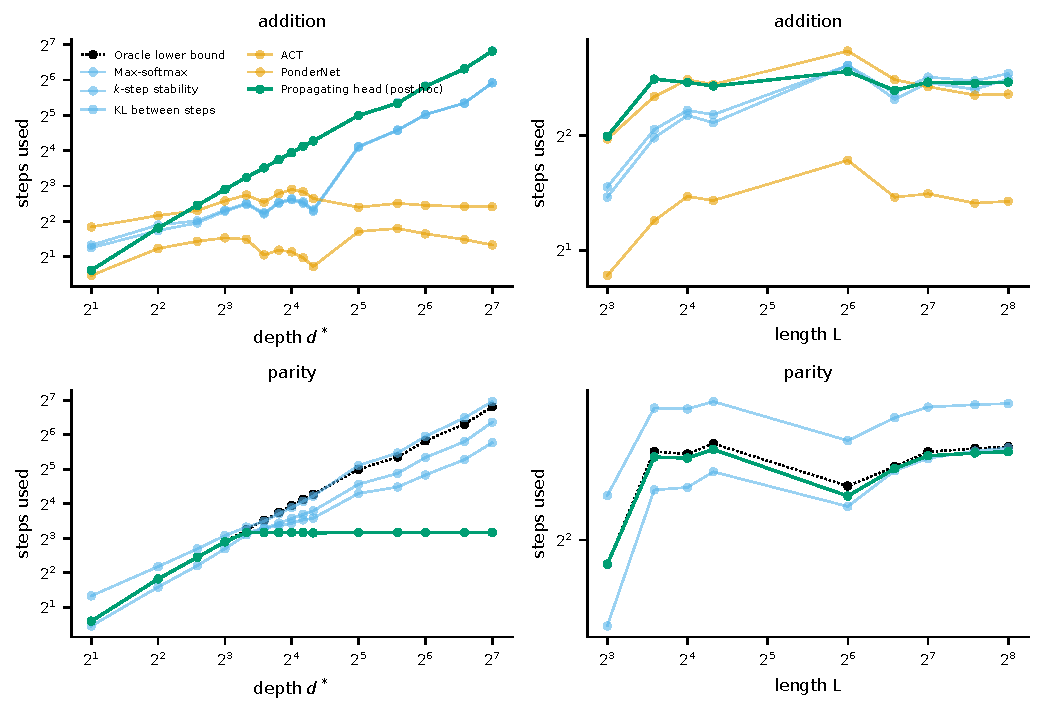
\includegraphics[width=0.78\linewidth]{figures/fig4_steps_vs_depth_length.pdf}
  \caption{Steps used against depth (left) and length (right). The light-cone bound (dotted) grows
  with depth only. Per-position rules on addition track it; pooled gates stay flat.}
  \label{fig:steps}
\end{figure}

\paragraph{Premature stopping is not premature error (H2).} Global convergence rules ($k$-step
stability and the KL divergence between steps) halt before $\mathrm{LB}(x)$ on 75\% of OOD-depth and
50\% of OOD-both addition instances (\cref{tab:premature}), yet remain 99.8\% accurate; their
premature-\emph{error} rate, pooled over the deep splits, is 0.1\%, against 18--23\% for ACT, PonderNet
and the joint pooled head. This is exactly the gap \cref{thm:lb} leaves open: the answers are
uncertified, but the data do not contain the flip partner. The backbone's default guess for a pending
digit is usually right, and while a carry wave is still travelling the hidden state keeps changing, so
convergence is a good proxy for completion. Parity shows the same effect in its sharpest form: one step
before the bound, a position has seen every bit of its segment and only the closing delimiter is
outside its window, so the natural guess (``no further bits'') is right on the actual input. This is
why the stable oracle and ACT can be accurate on parity OOD-depth while halting before the bound. The hidden-state-change rule, whose threshold is set on
short inputs, halts after about four steps on OOD-both and is correct on 42.7\%. On parity, where outputs
keep flipping as information arrives, confidence is misleading: max-softmax halts before the bound on
91\% of OOD-depth instances and is correct on 51\%; on OOD-both it is correct on 0.8\%. Only the KL rule
partly survives (94\% on OOD-depth, 57\% on OOD-both). Both H1 and H2 hold, so Gate G2 passes.

\begin{table}[t]
  \centering
  \caption{Premature-stop rate (\%): fraction of instances halted before the light-cone bound
  $\mathrm{LB}(x)$. Such answers are uncertified (\cref{thm:lb}), though not necessarily wrong.}
  \label{tab:premature}
  \scriptsize
  \setlength{\tabcolsep}{3pt}
  \resizebox{\linewidth}{!}{\begin{tabular}{lrrrr}
\toprule
 & \multicolumn{2}{c}{addition} & \multicolumn{2}{c}{parity} \\
 & OOD-depth & OOD-both & OOD-depth & OOD-both \\
\midrule
Fixed $T$ & 100.0 \tiny{[100.0, 100.0]} & 100.0 \tiny{[100.0, 100.0]} & 100.0 \tiny{[100.0, 100.0]} & 100.0 \tiny{[100.0, 100.0]} \\
Max-softmax & 0.0 \tiny{[0.0, 0.0]} & 0.0 \tiny{[0.0, 0.0]} & 90.8 \tiny{[89.9, 91.7]} & 98.2 \tiny{[97.5, 98.8]} \\
Entropy & 0.0 \tiny{[0.0, 0.0]} & 0.0 \tiny{[0.0, 0.0]} & 99.2 \tiny{[98.9, 99.5]} & 100.0 \tiny{[100.0, 100.0]} \\
$k$-step stability & 74.7 \tiny{[73.3, 76.0]} & 49.7 \tiny{[47.4, 51.9]} & 86.2 \tiny{[85.2, 87.3]} & 85.5 \tiny{[84.0, 87.1]} \\
KL between steps & 74.7 \tiny{[73.3, 76.0]} & 49.7 \tiny{[47.4, 51.9]} & 49.2 \tiny{[47.7, 50.7]} & 28.5 \tiny{[26.5, 30.6]} \\
Hidden-state change & 0.0 \tiny{[0.0, 0.0]} & 100.0 \tiny{[100.0, 100.0]} & 81.1 \tiny{[79.9, 82.3]} & 100.0 \tiny{[100.0, 100.0]} \\
Max confidence (Fan et al.) & 0.0 \tiny{[0.0, 0.0]} & 0.0 \tiny{[0.0, 0.0]} & 0.0 \tiny{[0.0, 0.0]} & 0.0 \tiny{[0.0, 0.0]} \\
Correctness head (post hoc) & 75.3 \tiny{[73.9, 76.6]} & 99.6 \tiny{[99.3, 99.9]} & 100.0 \tiny{[100.0, 100.0]} & 100.0 \tiny{[100.0, 100.0]} \\
ACT & 100.0 \tiny{[100.0, 100.0]} & 100.0 \tiny{[100.0, 100.0]} & -- & -- \\
PonderNet & 75.5 \tiny{[73.5, 77.4]} & 100.0 \tiny{[100.0, 100.0]} & -- & -- \\
Correctness head (joint) & -- & -- & -- & -- \\
v1 GLWM gate & -- & -- & -- & -- \\
Completion head (post hoc) & 0.0 \tiny{[0.0, 0.0]} & 0.0 \tiny{[0.0, 0.0]} & 100.0 \tiny{[100.0, 100.0]} & 100.0 \tiny{[100.0, 100.0]} \\
Propagating head (post hoc) & 0.7 \tiny{[0.4, 0.9]} & 0.1 \tiny{[0.0, 0.1]} & 100.0 \tiny{[100.0, 100.0]} & 100.0 \tiny{[100.0, 100.0]} \\
Completion head (joint) & -- & -- & -- & -- \\
Propagating head (joint) & -- & -- & -- & -- \\
\bottomrule
\end{tabular}}
\end{table}

\paragraph{Per-position certificates on addition (H3).} On addition every per-position rule halts at
the light-cone bound on every split, with no premature stops and at least 99\% accuracy: max-softmax,
entropy, and all four completion-head variants use 13.5 steps on OOD-depth and 75.4--75.6 on OOD-both,
against 13.5 and 75.4 for the oracle $\mathrm{LB}(x)$. The reason is visible in the theory: a pending
addition digit has two equally plausible outputs (carry or no carry), so a calibrated decoder is
uncertain at exactly the positions that are not yet determined, and the minimum over positions is a
local certificate in the sense of \cref{cor:local}. A linear probe recovers the pending bit from the
hidden state with AUC above 0.999 on every split (\cref{tab:probes}). Per-position confidence on
addition therefore already implements the automaton of \cref{prop:automaton}, and a learned completion
head adds nothing: G3, which required a 10-point gain over the best baseline, fails on addition by
construction.

\paragraph{Completion heads on parity learn the clock.} On parity all completion heads halt after about
nine steps regardless of depth, close to the largest training depth, and are correct on 31--34\% of
OOD-depth and 0\% of OOD-both instances, well below ACT and PonderNet on OOD-depth. The joint and
propagating variants behave the same. In training
every position is done by step 10, so ``late'' and ``done'' are indistinguishable, and the parity
backbone's hidden state encodes elapsed time well enough for the head to use it. The propagating head
was designed to wait for its neighbours, but nothing in the training data forces it to: a neighbour is
also always done by step 10. This is the same failure as the pooled gates, moved from the input length
to the step count. G3 fails on parity as well. Following the pre-registered pivot, we read the results
as a map of when simple signals suffice rather than as a win for a new halting method.

\paragraph{Decoupling (H4) and compute.} Training a completion head jointly changes the backbone's
step-averaged ID-val accuracy by less than 0.02 points on both tasks, so the auxiliary target does not
distort the task solution. Gates that reweight the task loss do: relative to the base model, ACT lowers
it by 34 points and the v1 gate by 17 points on addition (86 points for the v1 gate on parity), because
steps after the learned halting point receive little task gradient. In
FLOPs, a completion head costs one pointwise MLP per position and step, and the cost of every rule is
dominated by the number of steps it takes (\cref{fig:compute}). Wall-clock savings are smaller at our scale:
with online early exit on 512 OOD-depth instances, max-softmax takes 19.8\,ms against 23.8\,ms for the
full budget, while the completion heads take 23.8 and 28.3\,ms, because checking a rule after every step
(a host synchronisation plus re-batching) costs about as much as the steps it saves
(\cref{tab:probes}). Turning certified halting into latency savings needs fused halting checks or
larger models whose step cost dominates.

\paragraph{Ablations.} Removing input re-injection (recall) leaves OOD-depth intact but destroys
OOD-both (stable oracle 0.6\%). Halving the width to 64 lowers the stable oracle to 95.2\% but
max-softmax to 48.0\%: with less capacity the decoder's confidence stops tracking the pending state.
Two convolutions per step ($r=2$) reach 100\% on both (\cref{tab:probes}). Single seed each.
The accuracy-versus-steps trade-off of every threshold is shown in \cref{fig:tradeoff}, and premature stopping as a function of depth in
\cref{fig:premature_depth} (\cref{app:results}).
